\documentclass [paper=a4, fontsize=11pt]{article}%[paper=a4, fontsize=11pt, twocolumn]{article}
\usepackage{amsmath,amsfonts,amsthm} % Math packages
\usepackage{graphicx}
\graphicspath{ {Images/} }
\title{Combining different model predictions to increase product classification performance}

\author{Kim Beunder (s0209074) \& Kevin Serrano (s1595040)}

\begin{document}

\maketitle
\begin{abstract}
	In e-commerce companies, the quality of product analysis depends heavily on the ability to accurately cluster similar products. Given a dataset from the OTTO company, multiple different learning algorithms are used to build of different classifiers. By combining the outputs (predictions) obtained it is possible to outstand the performance that would be otherwise achieved making use of only one classifier.
\end{abstract}
\section{Introduction}
Whether online or not when selling products it is useful to sort your products in categories. That way buyers have an easier time finding what they're looking for. It is tedious work to have to sort every item into a category by hand, especially if hundreds of new items are added at once. Unfortunately it is rather difficult to automate the sorting and placing of products in a real store but for online stores it should be possible to automatically sort a new product in one of the existing categories. 

The Otto Group is one of the world’s biggest e-commerce companies, with subsidiaries in more than 20 countries, including Crate \& Barrel (USA), Otto.de (Germany) and 3 Suisses (France). The company sells millions of products worldwide every day, with several thousand products being added to the product line. A consistent analysis of the performance of the products is crucial. However, due to our diverse global infrastructure, many identical products get classified differently. Therefore, the quality of our product analysis depends heavily on the ability to accurately cluster similar products. The better the classification, the more insights we can generate about our product range.

There are multiple learning algorithms which could help with this task, each with their own strengths and the trick will be to determine which algorithm will be most suitable for the classification of Otto products. So the question that needs to be asked is:
\begin{center}
\textbf{Which learning algorithm is most suited for the sorting of products into categories and with what settings will the performance be optimal?}
\end{center}
To answer this question, we also pose several sub-questions to help define the criteria of the learning algorithm.
\begin{center}
\begin{enumerate}
\item How accurate can the algorithm be? How many items will be wrongly classified?
\item How long will the trained system need to categorize a new item?
\end{enumerate}
\end{center}
Research will be done to find promising learning algorithms for this specific situation. The top ones will be implemented, trained and tested. For each of these the above sub-questions will be answered. Based on the answers it will be discussed which of the tested algorithms is best suited for the classifying of Otto products.
\section{Otto Group Product Classification Challenge}
\subsubsection{Data}
For this competition, a dataset with 93 features for more than 200,000 products is provided. The objective is to build a predictive model which is able to distinguish between our main product categories. The winning models will be open sourced.

There are nine categories for all products. Each target category represents one of our most important product categories (like fashion, electronics, etc.). The products for the training and testing sets are selected randomly.
\subsubsection{Evaluation}
Submissions are evaluated using the multi-class logarithmic loss. Each product has been labeled with one true category. For each product, you must submit a set of predicted probabilities (one for every category). The formula is then,

$$ logloss=-\frac{1}{N}\sum_{i=1}^{N} \sum_{j=1}^{M}y_{ij}\log(p_{ij}) $$

where $N$ is the number of products in the test set, $M$ is the number of class labels, $log$ is the natural logarithm, $y_{ij}$ is $1$ if observation $i$ is in class $j$ and $0$ otherwise, and $p_{ij}$ is the predicted probability that observation $i$ belongs to class $j$.
\section{Related Work}
Competitors of this challenge share some of their proposals/solutions in the Otto challenge forum. They make use of different techniques in order to get a high score on the leaderboard. Some of them include:
\begin{itemize}
	\item Preprocessing data (tf-idf or log)
	\item Hyper-parameter tuning
	\item Classifier calibration (post-processing)
	\item Combining multiple different learning algorithms
\end{itemize} 

Some of this competitors have considerably good experience regarding Machine Learning, therefore throughout these paper some of the methods previously mentioned will be implemented and compared with the results obtained.

\section{Research and Analysis}
\subsection{Data Analysis}

The data that is made available to develop a classifier is made up of a training set with 61878 items and a testing set with 144368 items. Each item has an ID, 93 features and a label (only in the training set). It is not known what the features represent, there are simply 93 of them and their value ranges depending on which feature it is. The minimum value for each one is 0 and the maximum value an be found in figure \ref{fig:max_per_feature}. As it can be seen, maximum values per feature are different for the training and testing set.
\begin{figure}[h!]
    % \centering
    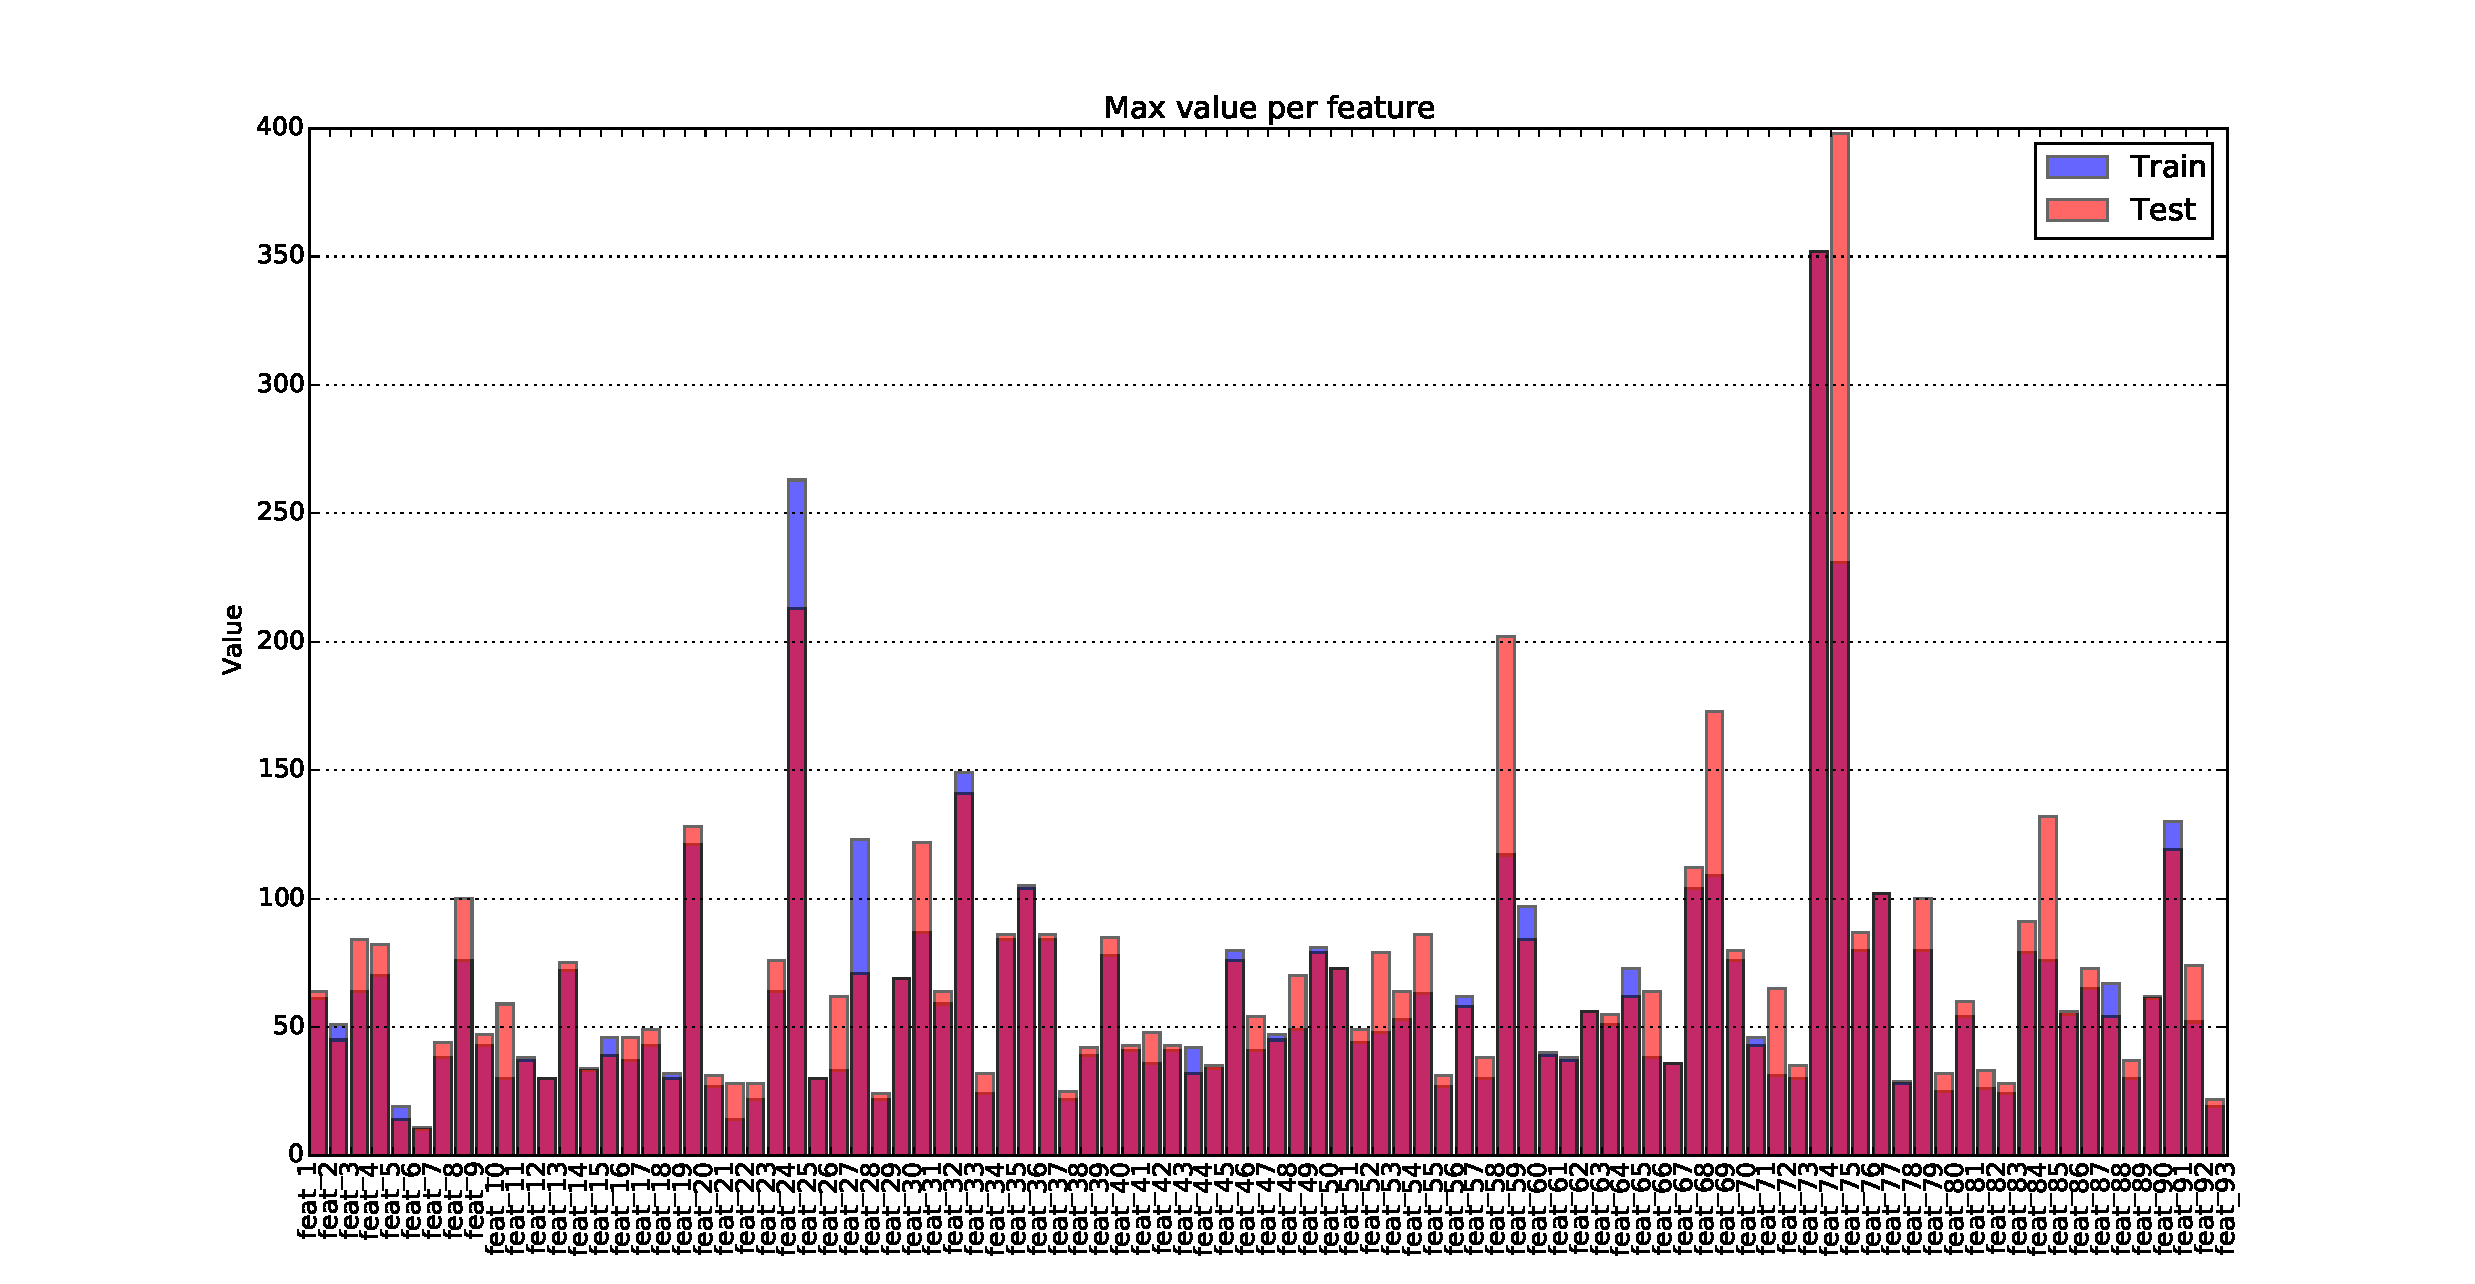
\includegraphics[trim={3.7cm 0cm 0.7cm 0.7cm},clip, width=1.1\textwidth]{max_per_feature}
    \caption{Maximum values per feature}
    \label{fig:max_per_feature}
\end{figure}

There are 9 different classes in which Otto wants its products classified. As with the features it is unknown what these classes represent.

As an attempt to visualize this high-dimensional data, the t-distributed stochastic neighbor embedding algorithm was used. It models each high-dimensional object by a two- or three-dimensional point in such a way that similar objects are modeled by nearby points and dissimilar objects are modeled by distant points.
\begin{figure}[h!]
    \centering
    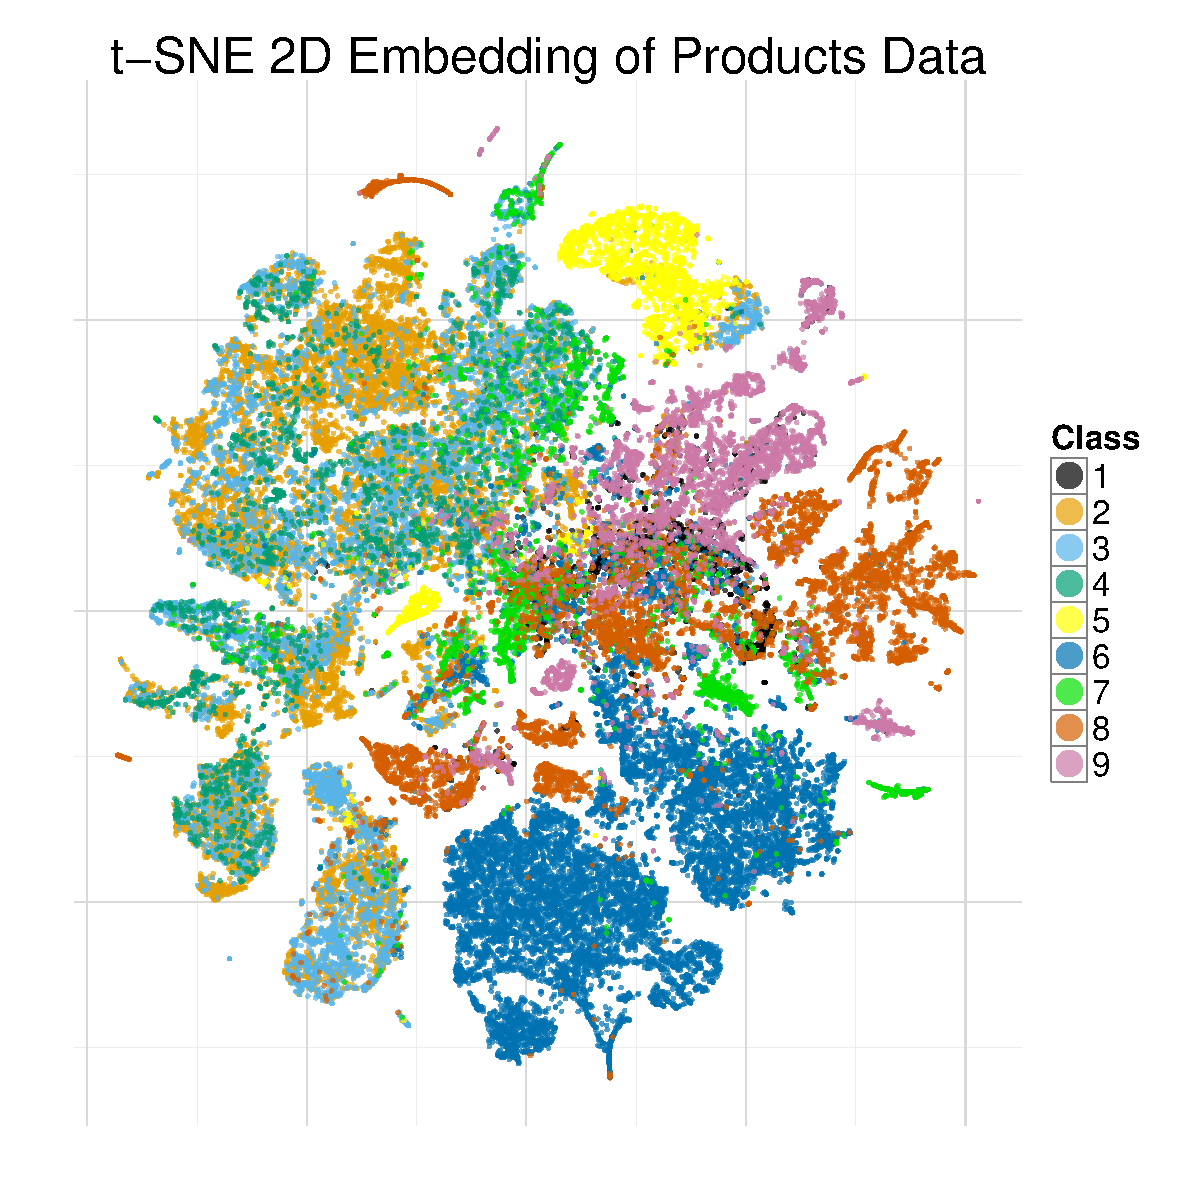
\includegraphics[width=0.9\textwidth]{tsne}
    \caption{t-distributed stochastic neighbor embedding}
    \label{fig:Tsne}
\end{figure}

From the result it can be seen that some samples will be most likely misclassified. Meaning that achieving a low logarithmic loss won't be easy.
\subsection{Research}
To find the most suitable machine learning algorithm for the classifying of Otto items we start by researching known algorithms. The most promising of the ones found are:
\begin{itemize}
\item Logistic regression
\item K-nearest neighbor
\item Random Forests
\item Gradient Boosting
\end{itemize}
All except Logistic Regression and K-nearest neighbor are ensemble methods, meaning that they are combinations of multiple machine learning algorithms. Ensemble methods often have better performance because they are more flexible due to the fact that they are combinations of several algorithms.\\
\subsubsection{Logistic Regression}
Logistic Regression is a direct probability model that was developed by statistician D. R. Cox in 1958. The probabilities describing the possible outcomes of a single trial are modeled, as a function of the predictor variables, using a logistic function. 

Logistic regression can be seen as a special case of generalized linear model and thus analogous to linear regression. However, The model of logistic regression is based on quite different assumptions, First, the conditional distribution $p(y|x)$ is a Bernoulli distribution rather than a Gaussian one, because the dependent variable is binary. Second, the estimated probabilities are restricted to $[0,1]$ through the logistic distribution function because it predicts the probability of the instance being positive.
\begin{figure}[h!]
	\centering
	\includegraphics[width=0.7\textwidth]{logistic_curve}
	\caption{Logistic function $\sigma(t)$}
	\label{fig:log_curve}
\end{figure}

Multinomial logistic regression is used when having multiple classes. This involves all classes uniformly by using the $softmax$ function (Bridle 1990). This boosts the weighted sum for one class through exponentiation and normalization so that it's corresponding output value is close to $1$.
\subsubsection{K-nearest neighbor}
 the k-Nearest Neighbors algorithm (k-NN) is a non-parametric method used for classification and regression. The input consists of the k closest training examples in the feature space and for k-NN classification the output is a class membership. A sample is assigned to the class most common among its $k$ nearest neighbors. k-NN is a type of lazy learning, where the function is only approximated locally and all computation is deferred until classification. It is one of the simplest of all machine learning algorithms. 
 
 It can be useful to assign weight to the contributions of the neighbors, so that the nearer neighbors contribute more than others. This can be achieved by using distant metrics (euclidean, manhattan, chebyshev).
\subsubsection{Random Forests}
Random Forests are similar to Bagging in the way that they have a similar basis. Both generate a number of trees of which each is constructed with a different sample of data and that give extra weight to points that were incorrectly classified. In Bagging the trees are independent from each other meaning newer trees are not dependent on earlier trees, they are constructed independently.

In Random Forests there is an extra layer of randomness in the method of constructing the classification trees. Instead of splitting each node and choosing the best from among all of the predictors, Random Forests split each node based on a randomly chosen subset of predictors. This might seem counter-intuitive but it actually appears to be robust against overfitting and it performs well.
\subsubsection{Gradient Boosting}
Gradient boosting is a machine learning technique for regression and classification problems, which produces a prediction model in the form of an ensemble of weak prediction models, typically decision trees.

Like other boosting methods, gradient boosting combines weak learners into a single strong learner, in an iterative fashion.
At each stage $1 \le m \le M$ of gradient boosting, it may be assumed that there is some imperfect model $F_m$. The gradient boosting algorithm does not change $F_m$ in any way; instead, it improves on it by constructing a new model that adds an estimator $h$ to provide a better model $F_{m+1}(x) = F_m(x) + h(x)$. In order to find $h$ we assume that a perfect solution would imply

    $$ F_{m+1} = F_m(x) + h(x) = y $$

or, equivalently,

    $$ h(x) = y - F_m(x) $$

Therefore, gradient boosting will fit $h$ to the residual $y - F_m(x)$. Like in other boosting variants, each $F_{m+1}$ learns to correct its predecessor $F_m$. Gradient boosting is a gradient descent algorithm; and generalizing it involves "plugging in" a loss function and its gradient.
\section{Implementation}
For the implementation of the learning algorithms we consider two options, MATLAB or Python. Both programming languages have existing have methods that support machine learning. However, we decided to use Python along with the \textbf{scikit-learn} library. The choice was made based on the simple and efficient tools this library offers and the fact that Python is a lightweight programming language, therefore it can process all the data we have significantly faster than MATLAB.

The process we followed can be summarized in the following steps:
\begin{enumerate}
	\item Create 'small' and 'big' training set.
	\item Inner split into training and test sets.
	\item Tune hyper-parameters using 'small' data.
	\item Train classifier using 'big' training data.
	\item Analyze performance results.
	\item Test classifier with original test set.
	\item Store probabilistic predictions for later use.
	\item Repeat steps 3. to 7. with a new learning algorithm
\end{enumerate}

First we begin by taking a small sample of the training dataset, 7\% to be precise, making sure the percentage of samples per class is preserved. Having now a small subset and the original set, we proceed to split them into inner training and test set (80/20). The small subset will be used for tuning the hyper-parameters of each learning algorithm. This is made using grid search which consists of making an exhaustive search over specified parameter values to find the combination which yields the best result. The grid search was conducted along with a 3-fold cross validation for a more reliable result. After tuning the hyper-parameters we proceed to train the classifier making use of the 'big' inner training set and measure its performance with the corresponding test set.

Until now, only the training set provided by OTTO was used. The next step consists on obtaining the probabilistic predictions making use of the test set originally provided. We store this predictions for a later analysis to improve the overall LogLoss performance.

\subsection{Logistic Regression}
\begin{table}[h!]
	\caption{The LogisticRegression parameters}
	\begin{tabular}{ | l | l | p{7cm} |}
		\hline
		\textbf{Parameter} & \textbf{Default} & \textbf{Description}\\
		\hline
		$C$ & 1.0 & Inverse of regularization strength; must be a positive float. Smaller values specify stronger regularization.\\
		\hline
		$penalty$ & l2 & ‘l1’ or ‘l2’. Used to specify the norm used in the penalization.\\
		\hline
		$class\_weights$ & None & Over-/undersamples the samples of each class according to the given weights. If not given, all classes are supposed to have weight one. The ‘auto’ mode selects weights inversely proportional to class frequencies in the training set.\\
		\hline
	\end{tabular}
	\label{table:LRdefaults}
\end{table}
The following set of hyper-parameter values was used:
\begin{itemize}
	\item C: 10\^-4:4
	\item penalty: ['l2', 'l1']
	\item class\_weights': [None, 'auto']
\end{itemize}
\subsubsection{Results}
\begin{table}[h!]
	\centering
	\caption{Grid search output}
	\begin{tabular}{ | l | c | c | c | c |}
		\hline
		$\bf{params_n}$ & \bf{C} &  \bf{penaly} & \bf{class\_weights} & \bf{log\_loss} \\ \hline
		$params_1$ & 0.2682 & 'l2' & 'auto' & 0.7952 \\ \hline
		$params_2$ & 0.2682 & 'l1' & 'auto' & 0.8175 \\ \hline
		$params_3$ & 0.0193 & 'l2' & None & 0.8245\\ \hline
		$params_4$ & 0.0719 & 'l2' & 'auto' & 0.8500 \\ \hline
		$params_5$ & 0.2682 & 'l2' & None & 0.8566 \\ \hline
	\end{tabular}
	\label{table:LR_gs}
\end{table}
\vspace{2mm}
\begin{figure}[h!]
	\centering
	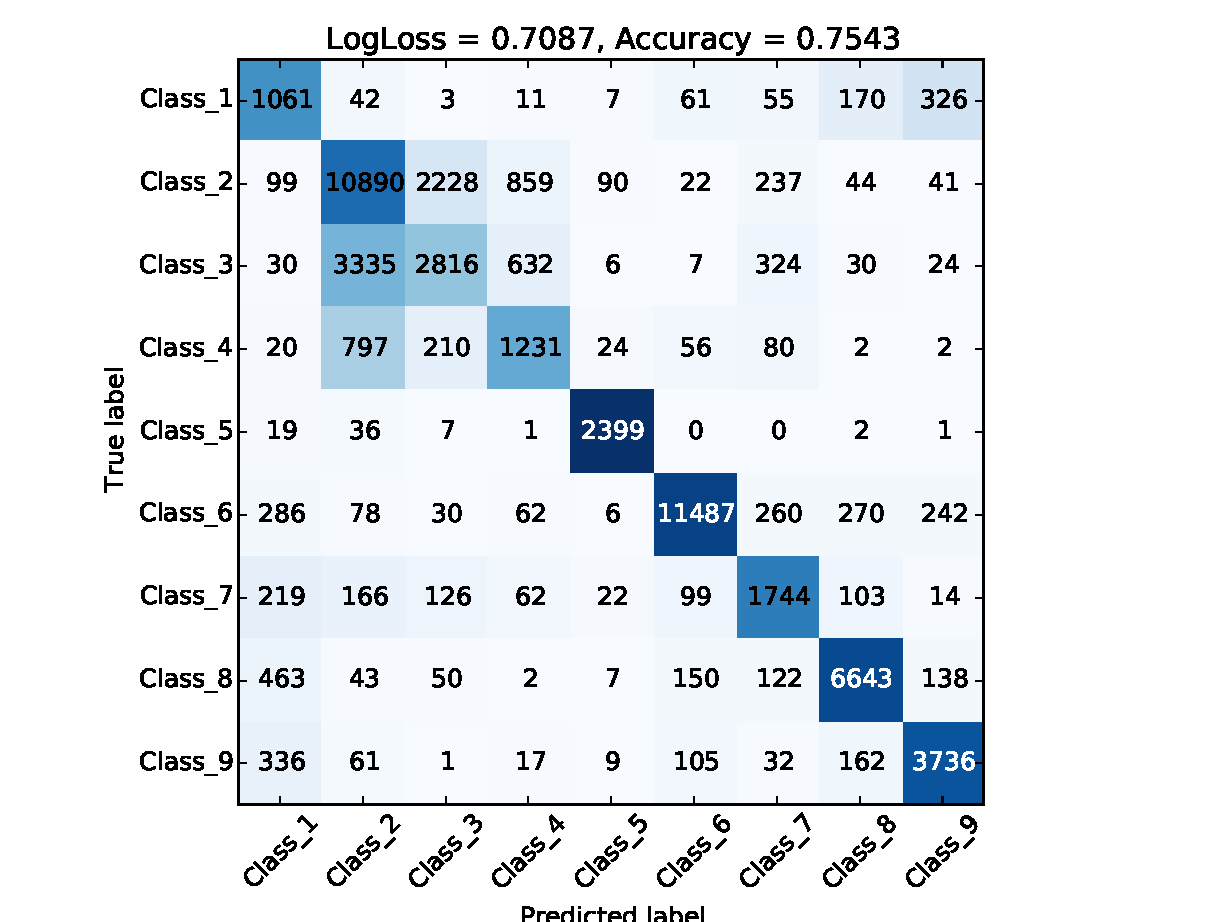
\includegraphics[width=0.7\textwidth]{LRcm_train}
	\caption{Logistic regression confusion matrix using training dataset}
	\label{fig:LRcm_train}
\end{figure}
\begin{figure}[h!]
	\centering
	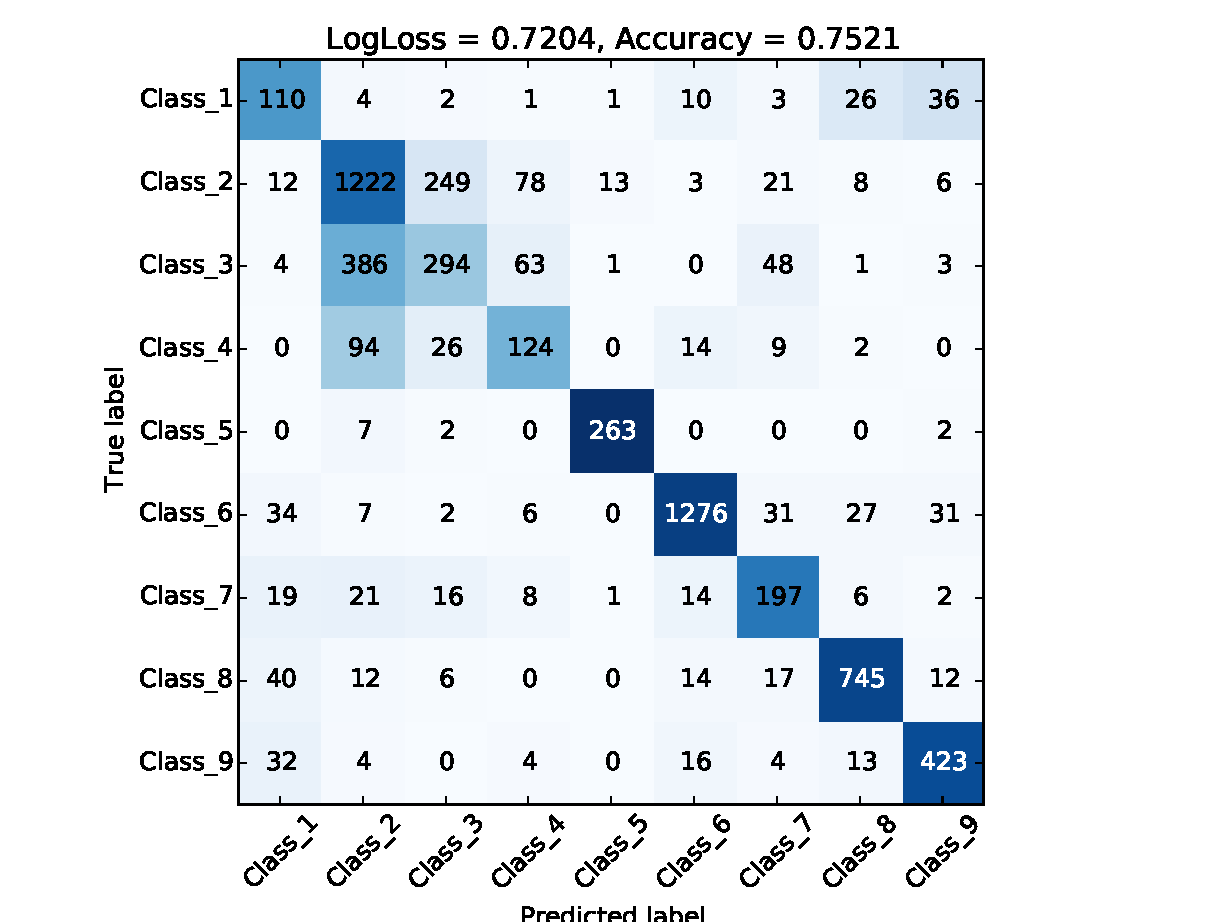
\includegraphics[width=0.7\textwidth]{LRcm_test}
	\caption{Logistic regression confusion matrix using testing dataset}
	\label{fig:LRcm_test}
\end{figure}
Performance using training and testing set is similar, but still not good enough. A lot of misclassifications are made among classes, specially between class 2 and 3.
\subsection{K-nearest neighbor}
\begin{table}[h!]
	\caption{The KNeighborsClassifier parameters}
	\begin{tabular}{ | l | l | p{7cm} |}
		\hline
		\textbf{Parameter} & \textbf{Default} & \textbf{Description}\\
		\hline
		$n\_neighbors$ & 5 & Number of neighbors to use.\\
		\hline
		$weights$ & uniform & weight function used in prediction.
		
		‘uniform’ : All points in each neighborhood are weighted equally. 
		
		‘distance’ : weight points by the inverse of their distance.\\
		\hline
		$algorithm$ & auto & Algorithm used to compute the nearest neighbors: ball\_tree, kd\_tree, brute (brute-force search) or auto. The last will attempt to decide the most appropriate algorithm based on the values passed to fit method.\\
		\hline
		$metric$ & minkowski & the distance metric to use for the tree.\\
		\hline
		$p$ & 2 & Power parameter for the Minkowski metric. When p = 1, this is equivalent to using manhattan\_distance, and euclidean\_distance for p = 2.\\
		\hline
	\end{tabular}
	\label{table:KNNdefaults}
\end{table}
The following set of hyper-parameter values was used:
\begin{itemize}
	\item n\_neighbors: [2, 3, 5, 7, 10, 15, 20]
	\item weights: ['uniform', 'distance']
	\item algorithm: ['ball\_tree', 'kd\_tree', 'brute']
	\item metric: ['minkowski']
	\item p: [1, 2, 3, 4, 5]
\end{itemize}
\subsubsection{Results}
\begin{table}[h!]
	\caption{Grid search output}
	\centering
	\begin{tabular}{ | l | c | c | c | c | c | c |}
		\hline
		$\bf{params_n}$ & \bf{n\_neighbors} & \bf{weights} & \bf{algorithm} & \bf{metric} & \bfseries{p}\  & \bfseries{log\_loss} \\ \hline
		$params_1$ & 20 & 'uniform' & 'brute' & 'minkowski' & 3 & 0.9871  \\ \hline
		$params_2$ & 20 & 'uniform' & 'kd\_tree' & 'minkowski' & 3 & 1.0305 \\ \hline
		$params_3$ & 15 & 'distance' & 'ball\_tree' & 'minkowski' & 3 & 1.0478 \\ \hline
		$params_4$ & 20 & 'uniform' & 'ball\_tree' & 'minkowski' & 5 & 1.1013 \\ \hline
		$params_5$ & 15 & 'distance' & 'ball\_tree' & 'minkowski' & 5 & 1.1176 \\ \hline
	\end{tabular}
\end{table}
%\vspace{2mm}
\begin{figure}[h!]
	\centering
	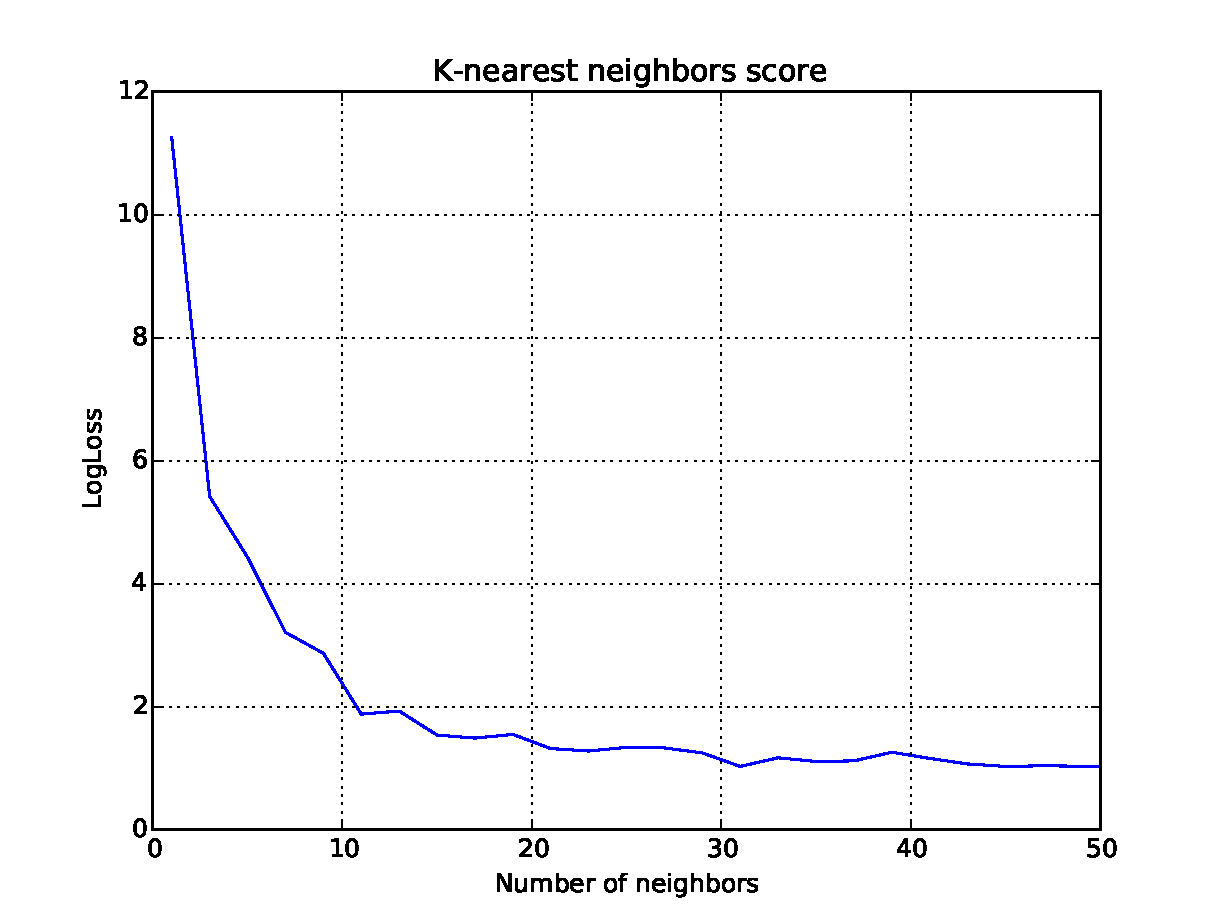
\includegraphics[width=0.8\textwidth]{KNN_scores}
	\caption{Scores varying the number of neighbors}
	\label{fig:KNN_scores}
\end{figure}
Figure \ref{fig:KNN_scores} was plotted by setting the $params_1$ obtained from the grid search and varying the number of neighbors. It can be appreciated that the LogLoss stops improving significantly passed the 30th neighbor.\\
\begin{figure}[h!]
	\centering
	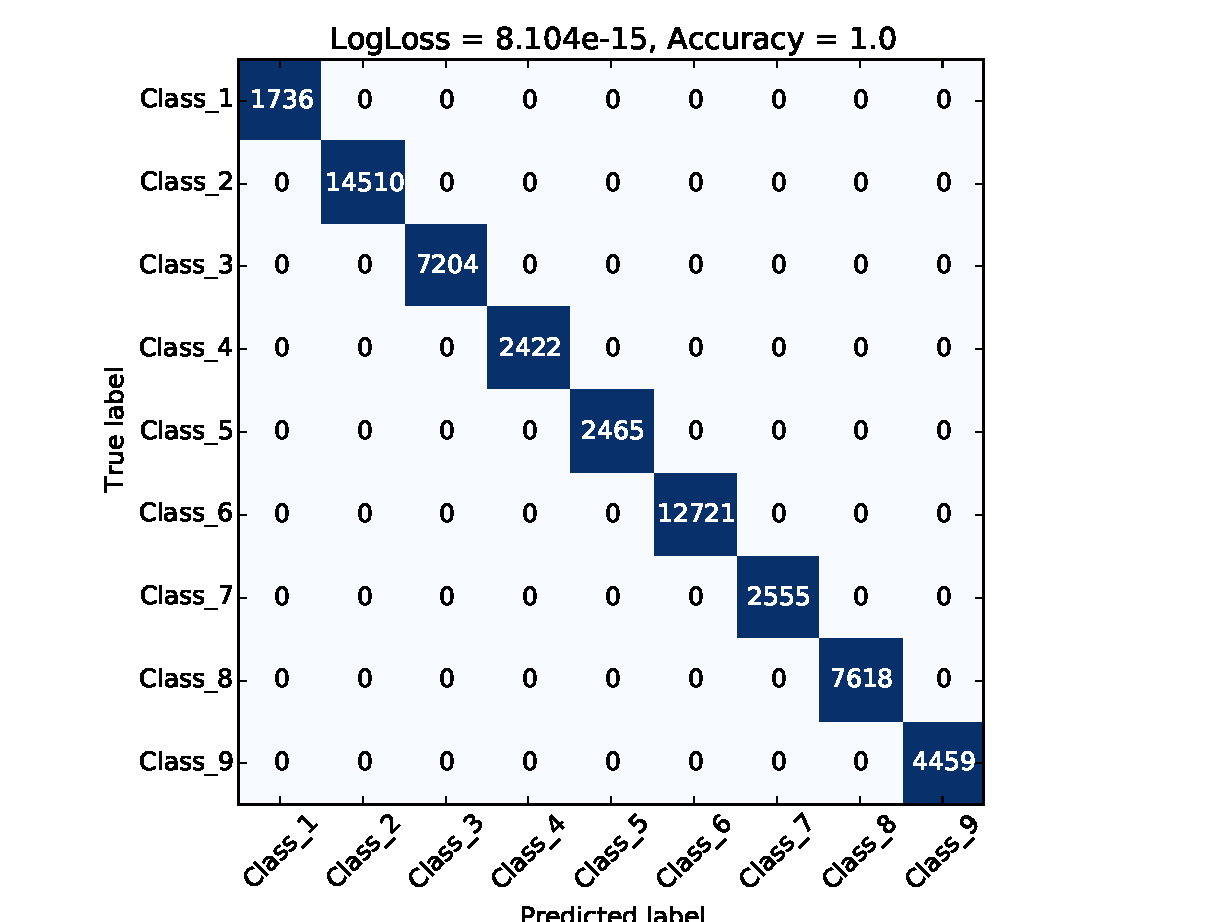
\includegraphics[width=0.7\textwidth]{KNNcm_train}
	\caption{k-NN confusion matrix using training dataset}
	\label{fig:KNNcm_train}
\end{figure}
\begin{figure}[h!]
	\centering
	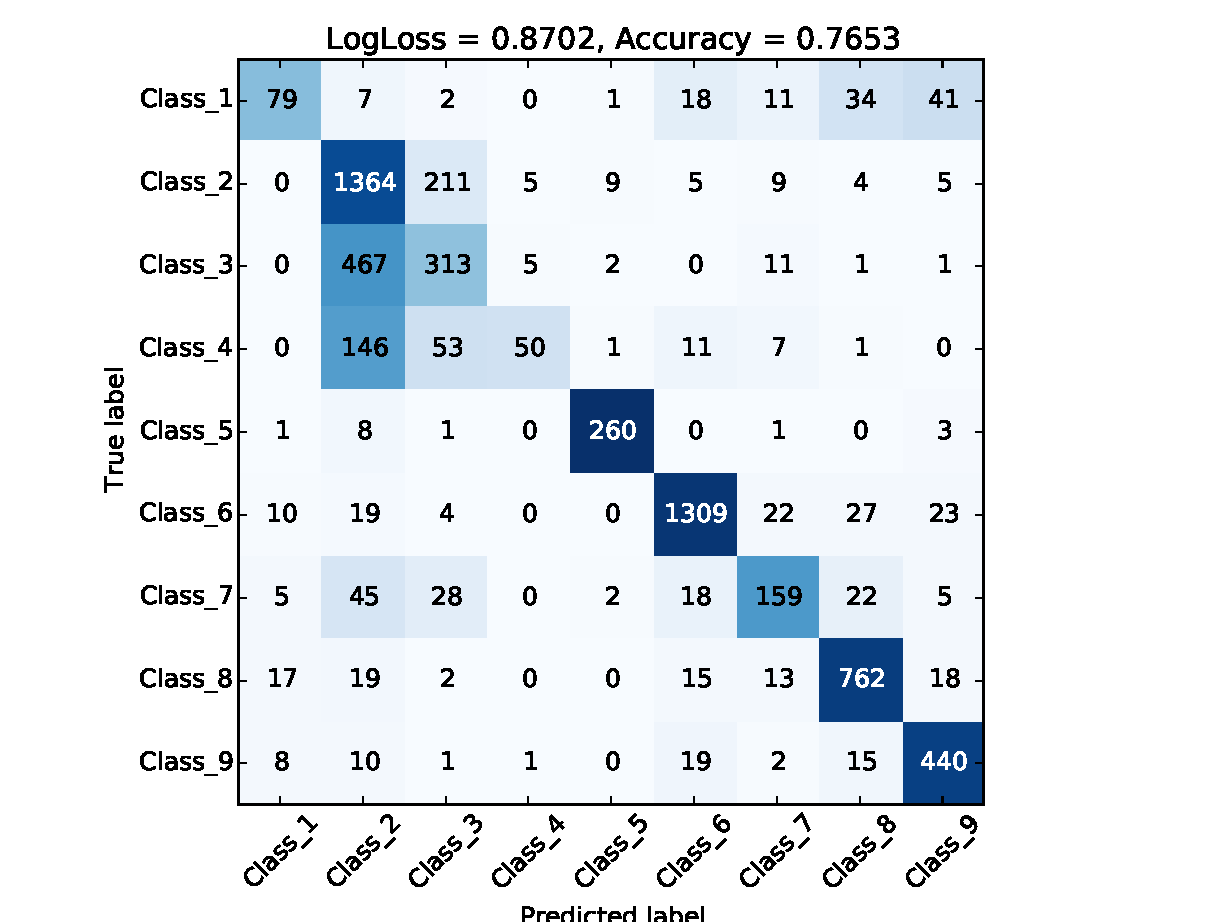
\includegraphics[width=0.7\textwidth]{KNNcm_test}
	\caption{k-NN confusion matrix using testing dataset}
	\label{fig:KNNcm_test}
\end{figure}\\
Because of the nature of the algorithm, measuring performance over the training set will always output a perfect accuracy because the points evaluated are exactly the same. The confusion matrix using the testing set gives us interesting results and an insight on how the data is arranged despite it's high dimensionality. There are lots of neighboring points between class 2, 3, and 4 which makes them the hardest classes to classify.\\
\subsection{Random Forests}
\begin{table}[h!]
	\caption{The RandomForestClassifier parameters}
	\begin{tabular}{ | l | l | p{7cm} |}
		\hline
		\textbf{Parameter} & \textbf{Default} & \textbf{Description}\\
		\hline
		$n\_estimators$ & 10 & Number of trees in the forest\\
		\hline
		$criterion$ & gini & Function to measure the quality of a split. "`gini"' for Gini impurity and "`entropy"' for information gain\\
		\hline
		$max\_depth$ & None &The maximum depth of the tree.\\
		\hline
		$max\_features$ & None & The number of features to consider when looking for the best split:\\
		\hline
	\end{tabular}
	\label{table:RFdefaults}
\end{table}
The following set of hyper-parameter values was used:\\
\begin{itemize}
	\item n\_estimators: 200
	\item criterion: ['gini', 'entropy']
	\item max\_depth: [2, 4, 6, 8],
	\item max\_features': [1.0, 0.7, 0.3, 0.1,'auto','sqrt','log2']
\end{itemize}
\subsubsection{Results}
\begin{table}[h!]
	\caption{Grid search output}
	\centering
	\begin{tabular}{ | l | c | c | c |}
		\hline
		$\bf{params_n}$ & \bf{criterion} &  \bf{mx\_features} & \bf{log\_loss} \\ \hline
		$params_1$ & 'gini' & 'auto' & 0.8646 \\ \hline
		$params_2$ & 'entropy' & 'auto' & 0.8969 \\ \hline
		$params_3$ & 'gini' & 'sqrt' & 0.9018 \\ \hline
		$params_4$ & 'gini' & 'log2' & 0.9336 \\ \hline
		$params_5$ & 'entropy' & 'log2' & 0.9635 \\ \hline
	\end{tabular}
\end{table}
The best parameters founds were selected, with exception of the number of estimators. This was varied in order to measure the performance vs the number of trees. It is important to remember that each tree in the forest is independent from one another and a large number of trees won't always imply that a better performance will be obtained even if testing over the training set.\\

Two different performance metrics were used, the LogLoss and the accuracy which as we can see in Figure \ref{fig:RFlog_loss} and Figure \ref{fig:RFaccuracy} behave differently. Accuracy is maintained relatively constant for both the training and testing set whereas the LogLoss provides us a more detailed visualization of the improvement in the predicted probabilities. Performance stops improving after 200 trees and no evident sign of overfitting is presented. If the only metric used was to be accuracy this fact couldn't be so easily seen leading to a less reliable score.\\
\begin{figure}[h!]
    \centering
    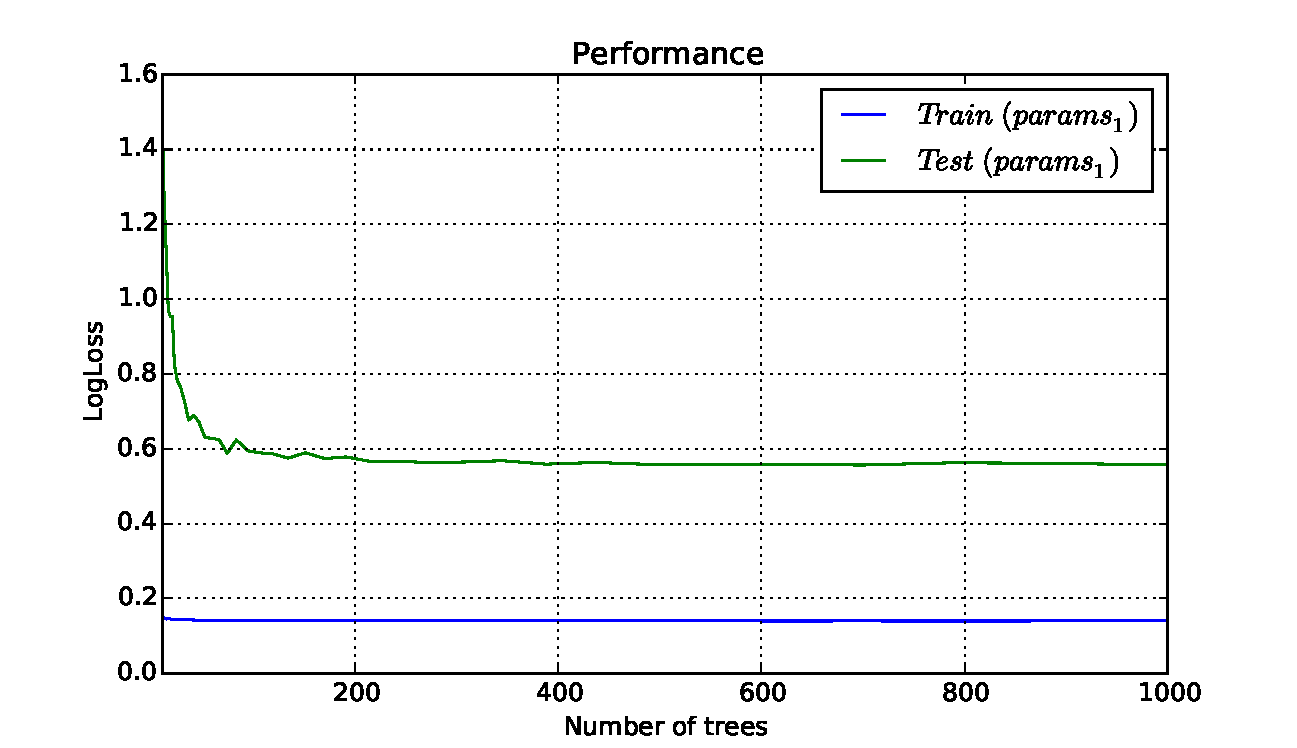
\includegraphics[width=1\textwidth]{RFlogloss}
    \caption{Performance using logarithmic loss as a metric}
    \label{fig:RFlog_loss}
\end{figure}\\
\begin{figure}[h!]
    \centering
    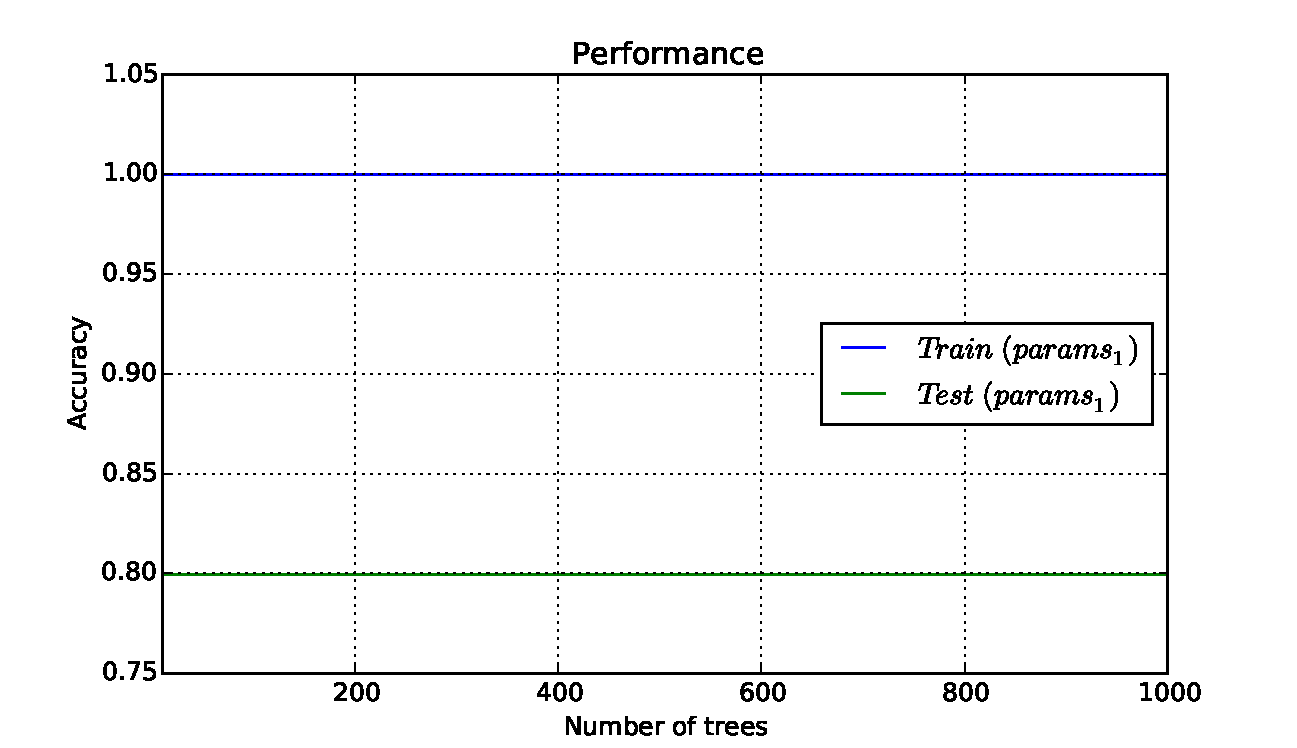
\includegraphics[width=1\textwidth]{RFaccuracy}
    \caption{Performance using accuracy as a metric}
    \label{fig:RFaccuracy}
\end{figure}\\
Confusion matrices were plotted using 400 as the number of estimators.
\begin{figure}[h!]
    \centering
    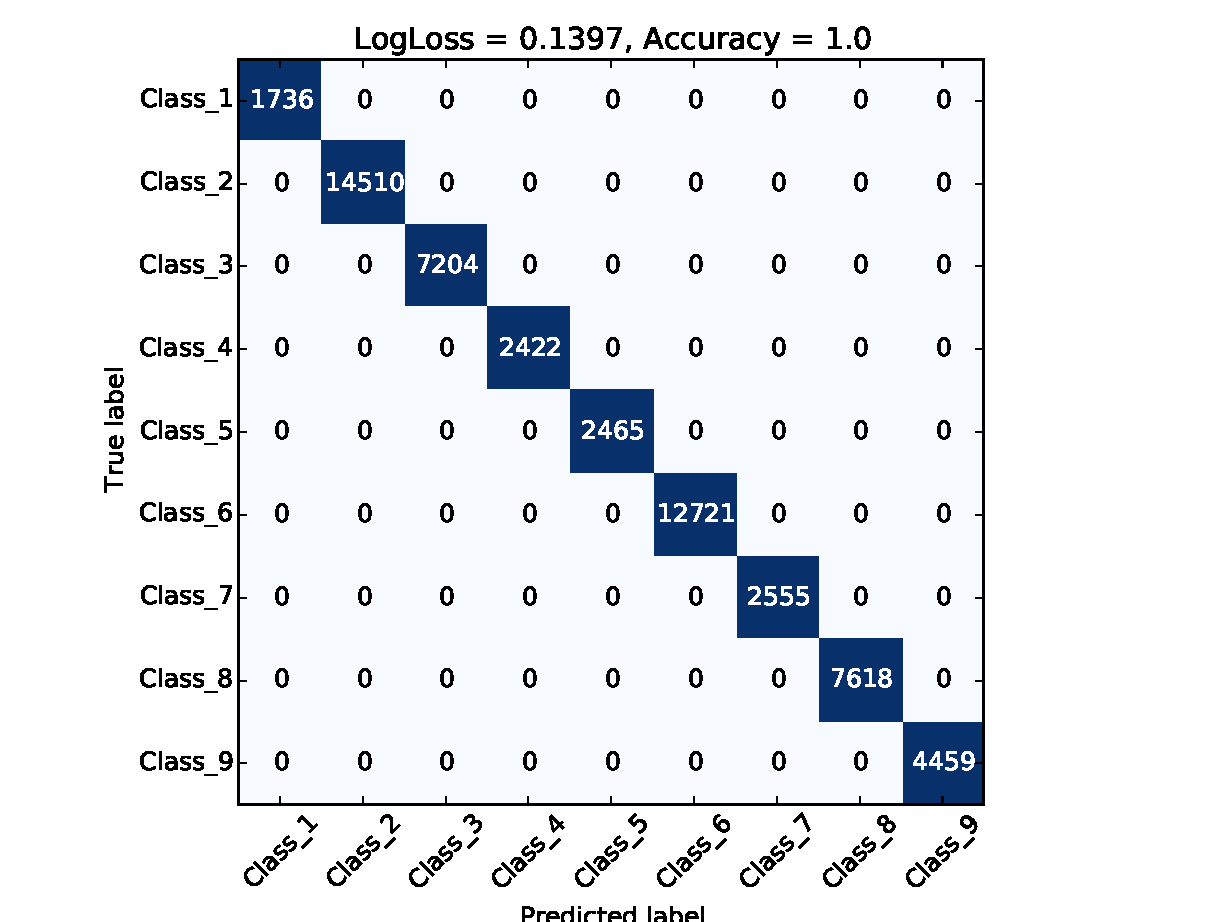
\includegraphics[width=0.7\textwidth]{RFcm_train}
    \caption{Random Forests confusion matrix using training dataset}
    \label{fig:RFcm_train}
\end{figure}
\begin{figure}[h!]
    \centering
    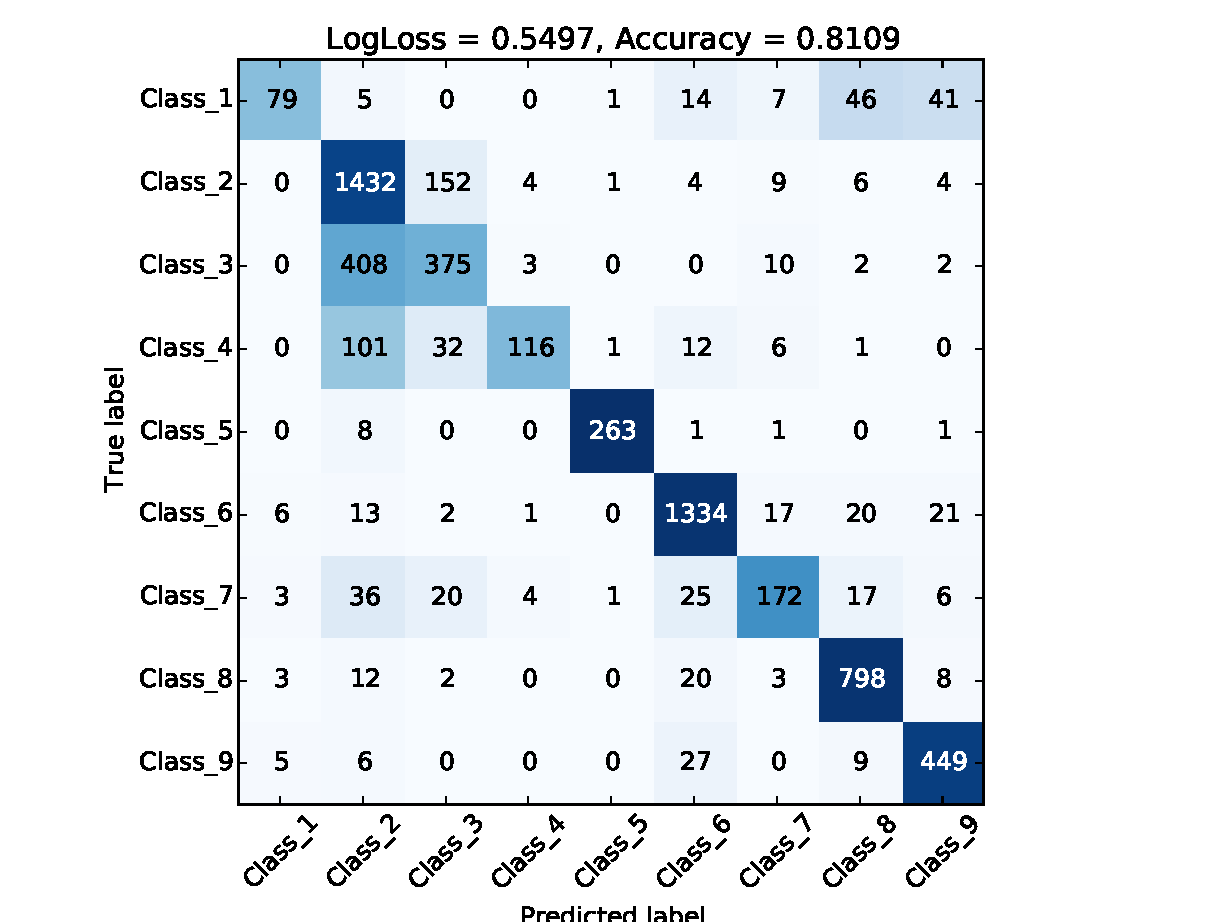
\includegraphics[width=0.7\textwidth]{RFcm_test}
    \caption{Random Forests confusion matrix using testing dataset}
    \label{fig:RFcm_test}
\end{figure}
\subsection{Gradient Boosting}
\begin{table}[h!]
	\caption{The GradientBoostingClassifier parameters}
	\begin{tabular}{ | l | l | p{7cm} |}
		\hline
		\textbf{Parameter} & \textbf{Default} & \textbf{Description}\\
		\hline
		$n\_estimators$ & 100 & The number of boosting stages to perform. Gradient boosting is fairly robust to over-fitting so a large number usually results in better performance.\\
		\hline
		$learning\_rate$ & 0.1 & learning rate shrinks the contribution of each tree by learning\_rate.\\
		\hline
		$max\_depth$ & 3 & The maximum depth limits the number of nodes in the tree.\\
		\hline
		$min\_samples\_leaf$ & 1 & The minimum number of samples required to be at a leaf node.\\
		\hline
		$max\_features$ & n\_features & The number of features to consider when looking for the best split.\\
		\hline
	\end{tabular}
	\label{table:GBdefaults}
\end{table}
The following set of hyper-parameter values was used:
\begin{itemize}
	\item learning\_rate: [0.1, 0.05, 0.02, 0.01],
	\item max\_depth: [2, 4, 6],
	\item min\_samples\_leaf: [3, 5, 9, 17],
	\item max\_features: [1.0, 0.7, 0.3, 0.1]
\end{itemize}
\subsubsection{Results}
\begin{table}[h!]
	\caption{Grid search output}
	\centering
	\begin{tabular}{ | l | c | c | c | c | c |}
		\hline
		$\bf{params_n}$ & \bf{l\_rate} &  \bf{mx\_depth} & \bf{m\_s\_leaf} & \bf{mx\_features} & \bf{log\_loss} \\ \hline
		$params_1$ & 0.05 & 4 & 17 & 0.7 & 0.6511 \\ \hline
		$params_2$ & 0.10 & 2 & 9 & 0.1 & 0.6756 \\ \hline
		$params_3$ & 0.05 & 4 & 17 & 0.1 & 0.7065 \\ \hline
		$params_4$ & 0.02 & 6 & 5 & 0.3 & 0.7143 \\ \hline
		$params_5$ & 0.05 & 4 & 5 & 0.3 & 0.7226 \\ \hline
	\end{tabular}
\end{table}
\begin{figure}[h!]
    \centering
    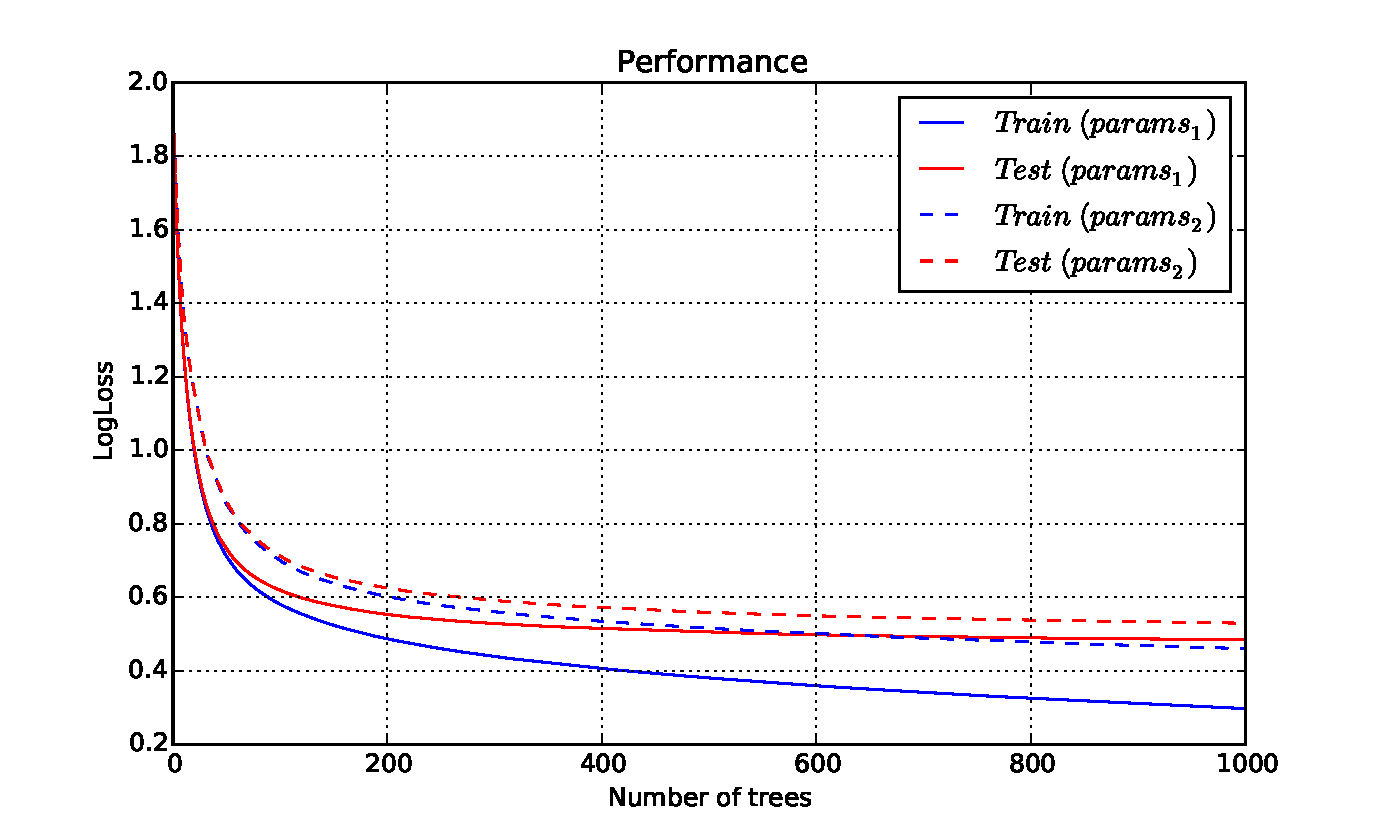
\includegraphics[width=0.86\textwidth]{GBlog_loss}
    \caption{Gradient boosting performance using logarithmic loss as a metric}
    \label{fig:GBlog_loss}
\end{figure}
\begin{figure}[h!]
    \centering
    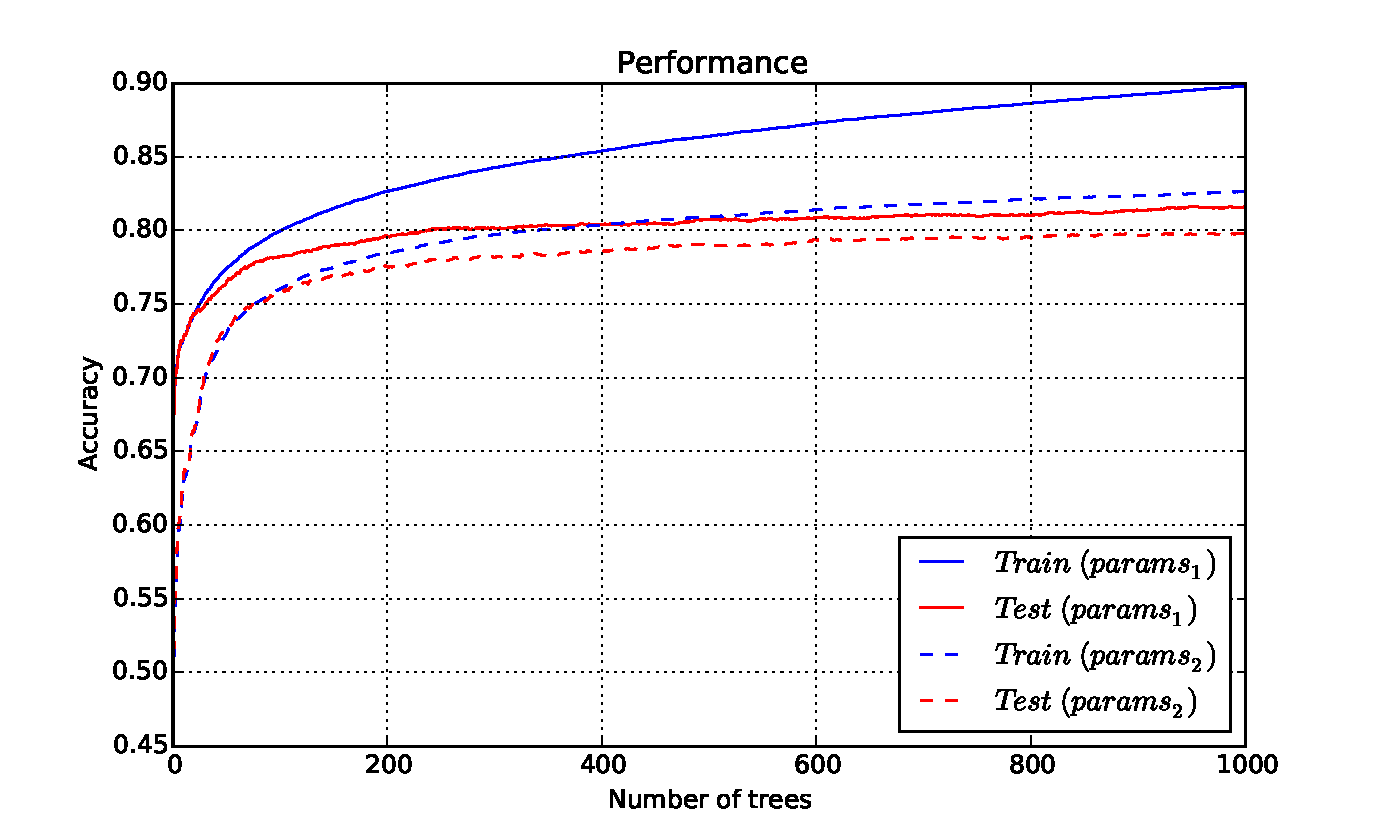
\includegraphics[width=0.9\textwidth]{GBaccuracy}
    \caption{Gradient boosting performance using accuracy as a metric}
    \label{fig:GBaccuracy}
\end{figure}
Knowing that, in boosting algorithms, each new classifier is an expert on the errors of its predecessor, we can compute the performance each time a new tree is added and plot it.

From figure \ref{fig:GBlog_loss} it can be seen that over-fitting is not present even with a large number of tree estimators. Differently from Random Forests, the accuracy changes with each tree that is added due to the fact that each new tree learns the errors of it's predecessor and a better output can be obtained. Performance improvement after the 500th tree is not significant and requires more memory and computation time.

\begin{figure}[h!]
    \centering
    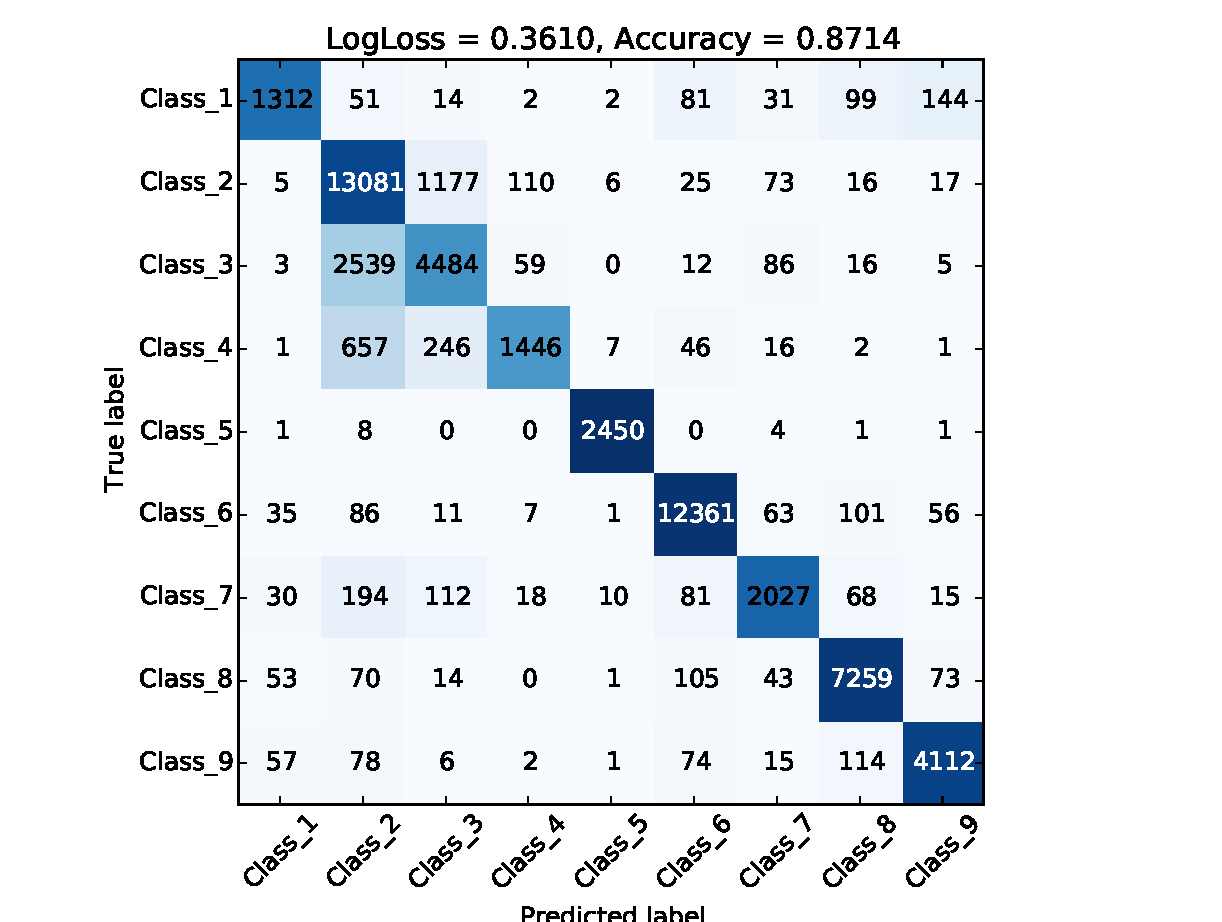
\includegraphics[width=0.69\textwidth]{GBcm_train}
    \caption{Gradient boosting confusion matrix using training set}
    \label{fig:GBcm_train}
\end{figure}
\begin{figure}[h!]
    \centering
    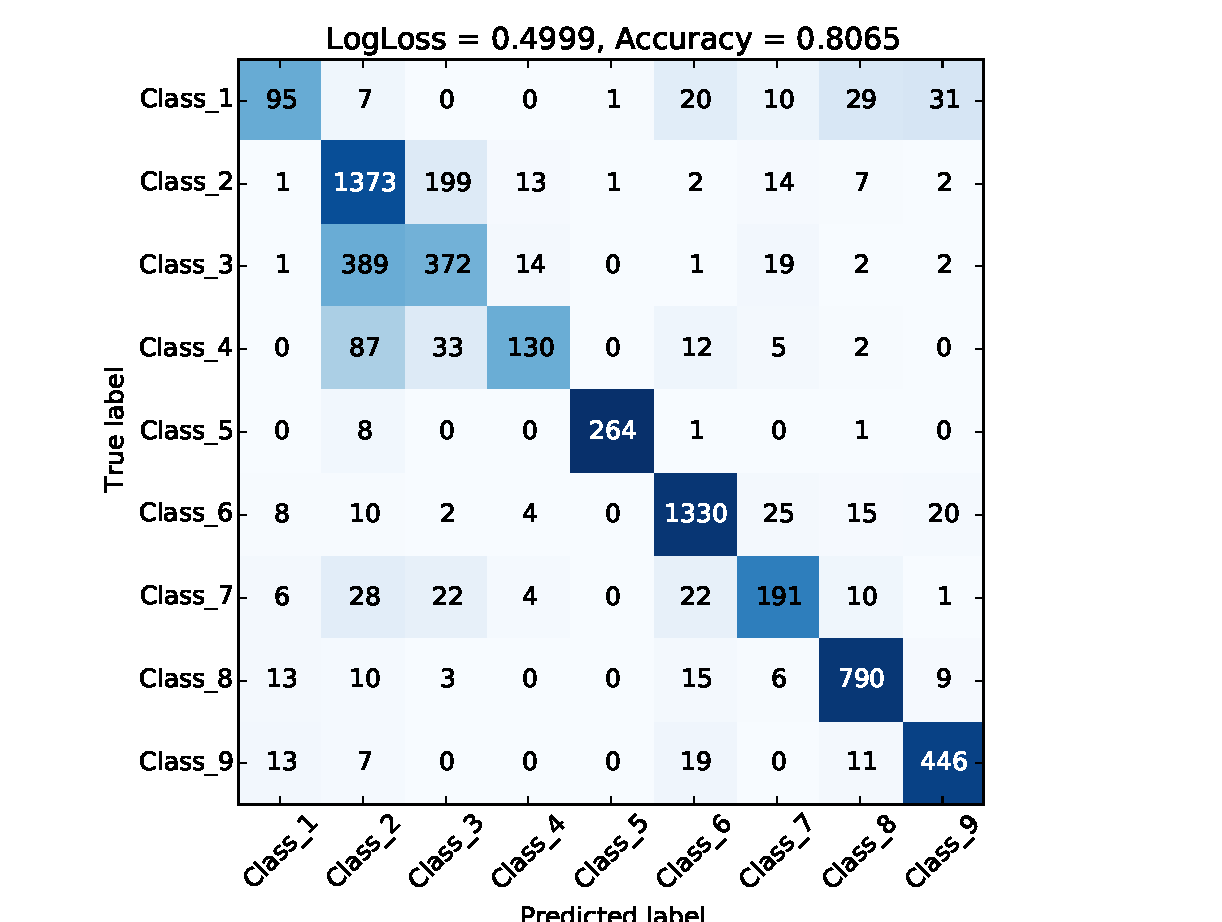
\includegraphics[width=0.7\textwidth]{GBcm_test}
    \caption{Gradient boosting confusion matrix using testing set}
    \label{fig:GBcm_test}
\end{figure}




\subsection{Combining predictions}
Having tested all the classifiers and obtaining ther respected probabilities we proceed to try to improve the overall performance by combining each of the predictions of the classifiers.

A brief summary can be visualized in Table \ref{table:summaryLogLoss}
\begin{table}[h!]
	\centering
	\caption{Test scores per classifier}
	\begin{tabular}{| l | c | c |}
		\hline
		\textbf{Classifier} & \textbf{Train} & \textbf{Test}\\
		\hline
		KNearestClassifier & 8.104e-15 & 0.8702 \\ \hline
		LogisticRegression & 0.7078 & 0.7204 \\ \hline
		RandomForestClassifier & 0.1397 & 0.5497 \\ \hline
		GradientBoostingClassifier & 0.3610 & 0.4978 \\ \hline
	\end{tabular}
	\label{table:summaryLogLoss}
\end{table}

From here we proceed to:
\begin{itemize}
	\item Average all 4 predictions
	\item Obtain weights to minimize LogLoss
\end{itemize}

From averaging predictions the final LogLoss is:

$$ LogLoss_{mean} = 0.5204 $$

Weights found after minimizing the LogLoss can be visualized in Figure \ref{fig:weights}
\begin{figure}[h!]
	\centering
	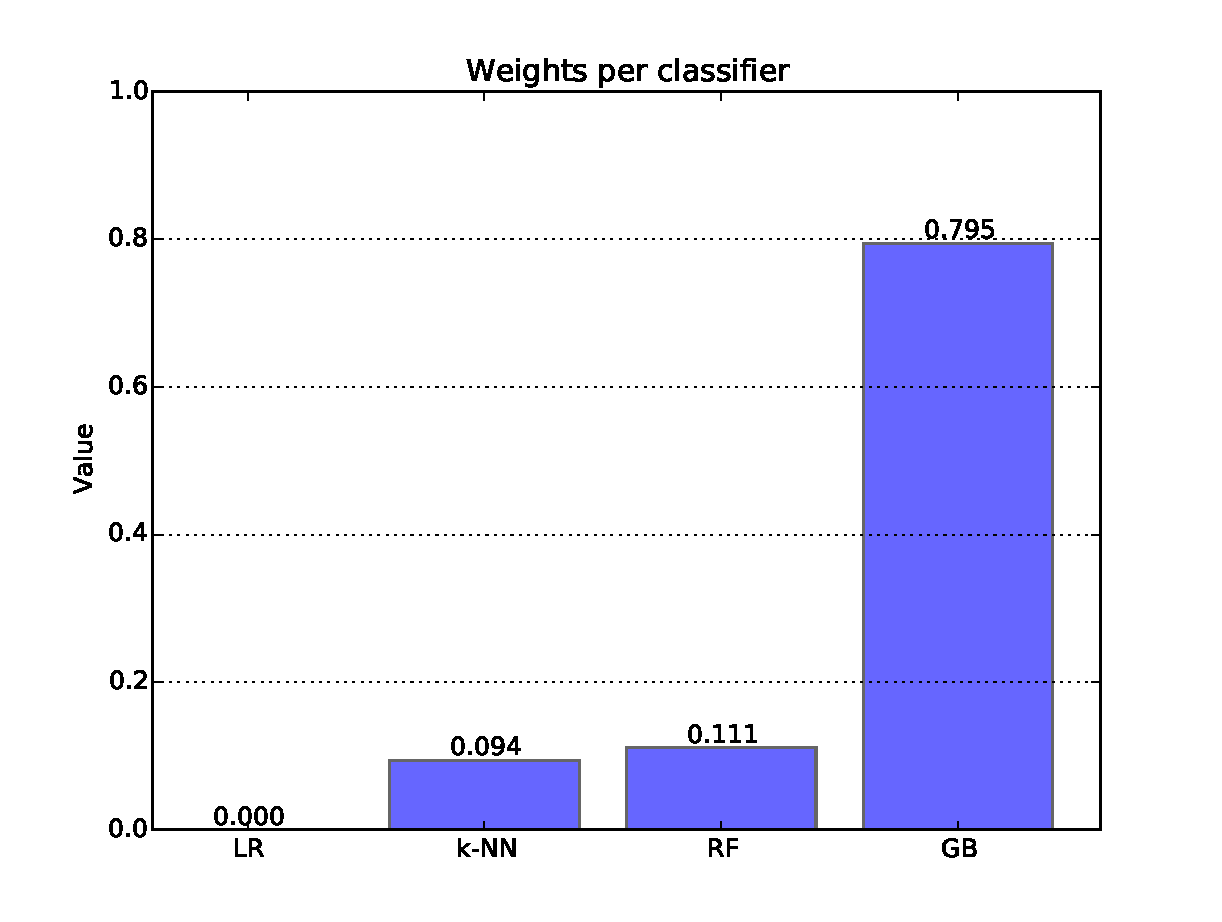
\includegraphics[width=0.8\textwidth]{weights}
	\caption{weights obtained from minimizing $LogLoss$ function}
	\label{fig:weights}
\end{figure}

$$ LogLoss_{weighted} = 0.4732 $$

The weights found can help ups identify which learning algorithms contribute the most to improving the LogLoss and which are practically useless. Indeed from Table \ref{table:summaryLogLoss} it can be foreseen that the output from Gradient Boosting would be one with most influence, however, even though the score using k-NN is the worst, it has nearly the same influence as Random Forest. Output obtained from Logistic Regression is practically useless given it's weight of $4.36e-7$.

\subsection{Computation time}
Even though no precise measurements for computation time in Table \ref{table:times} a general overview is presented where '$+++$' should be interpreted as 'fast' and '$---$' as 'slow'.

\begin{table}[h!]
	\centering
	\caption{Overview of training and predicting times}
	\begin{tabular}{| l | c | c |}
		\hline
		\textbf{Classifier} & \textbf{Training time} & \textbf{Predicting time}\\
		\hline
		KNearestClassifier & $+++$ & $---$ \\ \hline
		LogisticRegression & $++-$ & $++-$ \\ \hline
		RandomForestClassifier & $++-$ & $+--$ \\ \hline
		GradientBoostingClassifier & $+--$ & $++-$ \\ \hline
	\end{tabular}
	\label{table:times}
\end{table}

From the algorithms tested, the fastest to train is k-NN because it doesn't require training at all, and the slowest to train is gradient boosting. The fastest to predict is Logistic Regression followed by gradient boosting, and the slowest is k-NN because it has to make a search over all the dataset to find the k-nearest neighbors either by brute force or by some more efficient methods based on trees (ball tree or k-d tree).

It is interesting how both ensembles methods are inversely efficient, Random Forests is relatively fast to train but slow to predict and Gradient Boosting is the opposite. This is because in Random Forests th trees used are independent from each other with random samples from the data which makes training faster, however this trees have long depth which leads to a slow prediction. Gradient Boosting trees are connected and after the other making training slow, but the fact that this are weak learners (low depth trees) makes prediction faster. 
\section{Discussion}
Having analyzed multiple algorithms and their performances we can give an answer to the initial research question.
\begin{center}
	\textbf{Which learning algorithm is most suited for the sorting of products into categories and with what settings will the performance be optimal?}
\end{center}
While it is true that a single algorithm will perform better than others, results obtained in this paper indicate that combining outputs of multiple different learning algorithms lead to an increase in probability prediction performance. Even when the score of a certain learning algorithm is not as good as others one shouldn't underestimate it's possible influence to achieve a better result when combining them.

Winning competitors posted their approach, the two best scores implementations were based on stacking (stacked generalization) introducing the concept of meta learner. It can be seen as a more sophisticated version of cross-validation, exploiting a strategy which combines the individual models instead of picking the best one out the cross-validation results. The key idea is to perform cross-validation for the training and testing of base classifiers, then the predictions are used as the inputs, and the correct responses as the outputs to train a meta (higher level) classifier.

\begin{figure}[h]
	\centering
	\includegraphics[width=0.7\textwidth]{stackingschema}
	\caption{Stacking's schema of 2nd place winner}
	\label{fig:stacking}
\end{figure}
Nonetheless, in a stacking schema computational time will be limited by the slowest algorithm in terms of training and prediction because the output from all classifiers has to be used for averaging, voting or as input for a meta learner.


\section{Conclusions}
Combining results relying on probabilistic estimates from different learning algorithms is a way of improving score in classification problems. Diversity of learning methods is important to consider as it helps the overall final result. A trade between accuracy and computing time has to be made, an increase in performance would most probably imply an increase in computational time.

\begin{thebibliography}{9}
\bibitem{scikit_learn} 
Pedregosa \textit{et al}. 
\textit{Scikit-learn: Machine Learning in Python}. 
JMLR 12, pp. 2825-2830, 2011.
 
\bibitem{stacking} 
Wolpert, David H. 
Stacked generalization, \textit{Neural Networks}.
Volume 5, Issue 2, Pages 241-259.

\bibitem{ML_Alpaydm} 
Alpaydm, Ethem.
\textit{Introduction to machine learning}.
Massachusetts Institute of Technology, 2010
 
\bibitem{kaggle} 
Kaggle Inc 2015.
\textit{Otto Group Product Classification Challenge}.
\\\texttt{https://www.kaggle.com/c/otto-group-product-classification-challenge}
\end{thebibliography}
\end{document}